\documentclass[tikz,border=12pt]{standalone}
\usepackage{graphicx}
\usepackage{amsmath,amssymb}
\usepackage{tikz}
\usetikzlibrary{arrows.meta,positioning,fit,calc,backgrounds}
\tikzset{
  box/.style={
    draw,
    very thick,
    rectangle,
    align=center,
    inner sep=8pt,
    minimum height=1.25cm,
    minimum width=3.1cm,
    font=\small,
  },
  wide/.style={box, minimum width=3.6cm},
  arr/.style={-{Stealth[length=2.6mm, width=2mm]}, thick},
  barr/.style={
    {Stealth[length=2.4mm, width=1.8mm]}-{Stealth[length=2.4mm, width=1.8mm]},
    thick,
  },
  lbl/.style={font=\scriptsize, inner sep=2pt, fill=white},
  group/.style={draw, dashed, inner sep=12pt},
}

\begin{document}
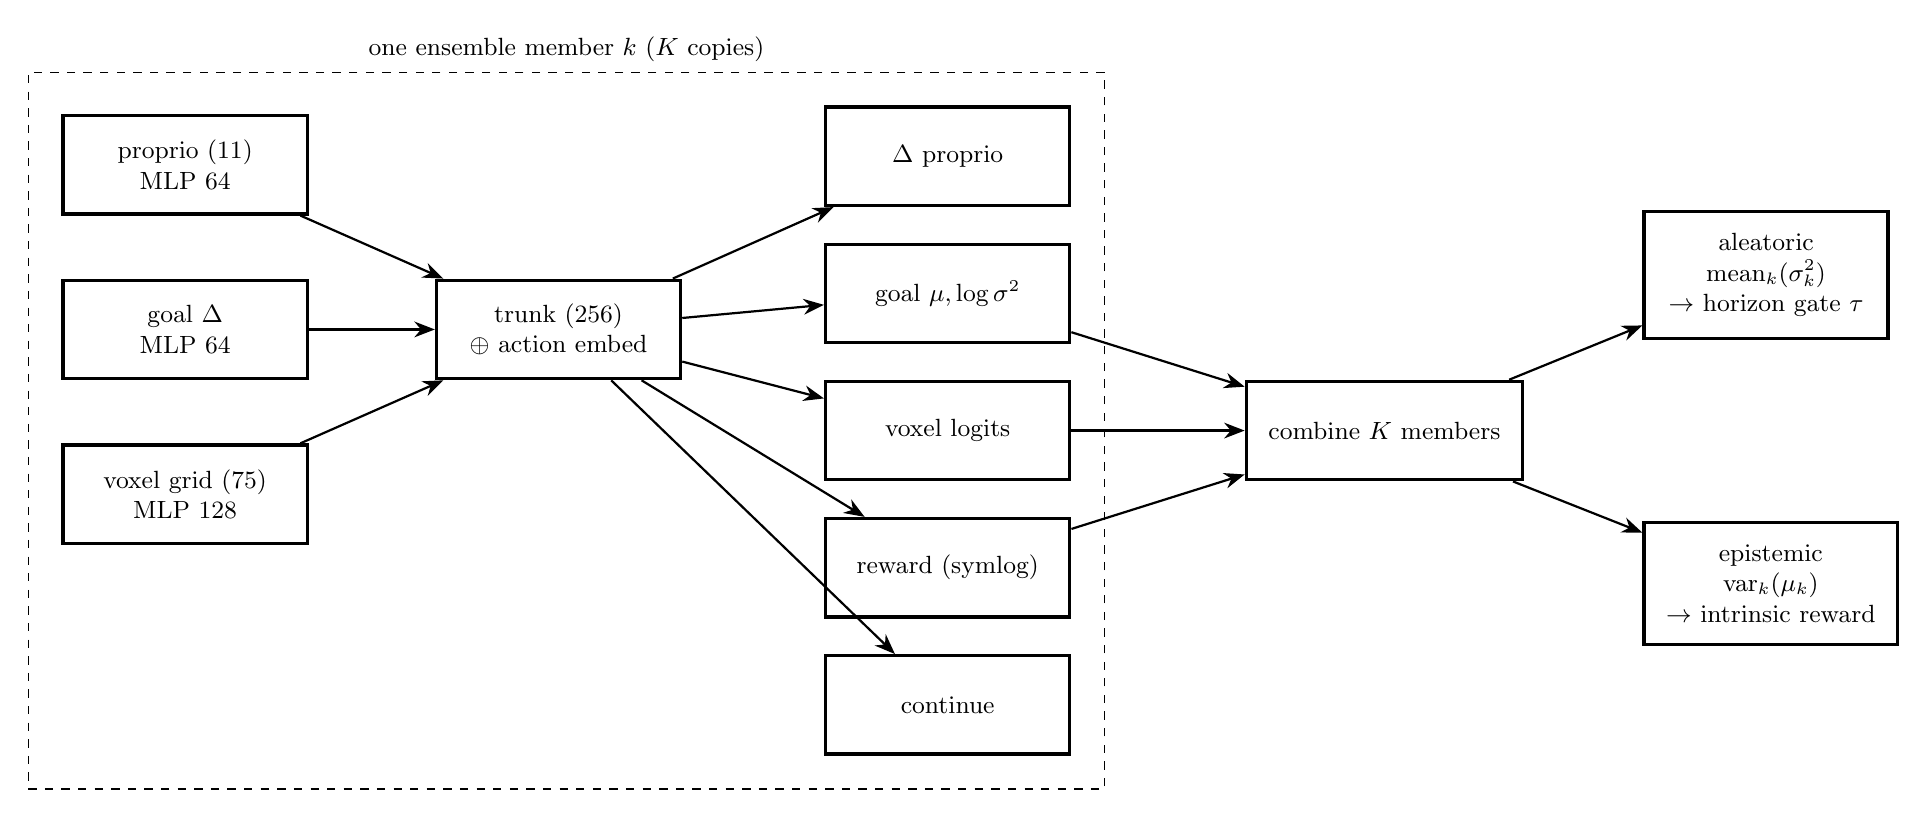
\begin{tikzpicture}[node distance=0.8cm and 1.3cm]
  \node[box] (p) {proprio (11)\\MLP 64};
  \node[box, below=of p] (g) {goal $\Delta$\\MLP 64};
  \node[box, below=of g] (v) {voxel grid (75)\\MLP 128};
  \node[box, right=1.6cm of g] (tr) {trunk (256)\\$\oplus$ action embed};
  \foreach \n in {p,g,v} \draw[arr] (\n) -- (tr);

  \node[box, right=1.8cm of tr, yshift=2.2cm] (h1) {$\Delta$ proprio};
  \node[box, below=0.45cm of h1] (h2) {goal $\mu,\log\sigma^2$};
  \node[box, below=0.45cm of h2] (h3) {voxel logits};
  \node[box, below=0.45cm of h3] (h4) {reward (symlog)};
  \node[box, below=0.45cm of h4] (h5) {continue};
  \foreach \n in {h1,h2,h3,h4,h5} \draw[arr] (tr) -- (\n);

  \node[group, fit=(p)(v)(tr)(h1)(h5), label={[font=\small]above:one ensemble member $k$ ($K$ copies)}] {};

  \node[box, right=2.2cm of h3] (ens) {combine $K$ members};
  \foreach \n in {h2,h3,h4} \draw[arr] (\n) -- (ens);
  \node[box, above right=0.5cm and 1.5cm of ens] (al) {aleatoric\\$\mathrm{mean}_k(\sigma_k^2)$\\$\to$ horizon gate $\tau$};
  \node[box, below right=0.5cm and 1.5cm of ens] (ep) {epistemic\\$\mathrm{var}_k(\mu_k)$\\$\to$ intrinsic reward};
  \draw[arr] (ens) -- (al);
  \draw[arr] (ens) -- (ep);
\end{tikzpicture}
\end{document}
